\documentclass[11pt,a4paper]{article}
\usepackage{fontspec}
\usepackage{bidi}
\newfontfamily\arabicfont[Script=Arabic,Scale=1.1]{Arial}
\setmainfont{Arial}
\usepackage{geometry}
\usepackage{graphicx}
\usepackage{booktabs}
\usepackage{float}
\usepackage{amsmath}
\usepackage{caption}
\usepackage{setspace}
\geometry{margin=2.5cm}
\captionsetup{font=small,labelfont=bf}
\setstretch{1.08}
\setlength{\parskip}{0.45em}
\setlength{\parindent}{0pt}
\setlength{\emergencystretch}{3em}

\begin{document}

\begin{center}
{\LARGE\arabicfont\RL{تحليل ارتباط درجات التقييم و\LR{PCA} و\LR{K-means}}\par}
\vspace{0.5em}
{\large\arabicfont\RL{17 أبريل 2026}\par}
\vspace{0.25em}
{\small\LR{p16\_review\_scores\_correlation\_pca\_kmeans.ipynb}\par}
\end{center}
\vspace{1em}

\begin{RTL}

\section*{{\arabicfont\RL{البيانات والمتغيرات}}}
يعرض هذا التقرير النتائج الفعلية المستخرجة من دفتر التحليل الحالي. وقد أُجري العمل على \textbf{63{,}871} إعلاناً تتوفر لها قيم كاملة في سبعة متغيرات من متغيرات درجات التقييم، وهي: الدرجة العامة، والدقة، والنظافة، وتسجيل الوصول، والتواصل، والموقع، والقيمة مقابل السعر.

يهدف هذا التحليل إلى توصيف البنية المشتركة بين هذه المتغيرات، ثم اختزالها إلى أبعاد مركبة يسهل تفسيرها، وأخيراً تقسيم الإعلانات إلى مجموعات متجانسة انطلاقاً من تموضعها في الفضاء العاملي. وبذلك يجمع التقرير بين الوصف الارتباطي، والاختزال البعدي، والتصنيف غير المراقب ضمن مسار تحليلي واحد.

\section*{{\arabicfont\RL{مخطط سير العمل}}}
يُلخّص الشكل التالي سير العمل التحليلي من تحميل ملف الإدخال إلى إنتاج الجداول والرسوم النهائية. وقد أُدرج المخطط اعتماداً على الرسم المولَّد سابقاً ضمن ملفات المشروع.

\begin{figure}[H]
    \centering
    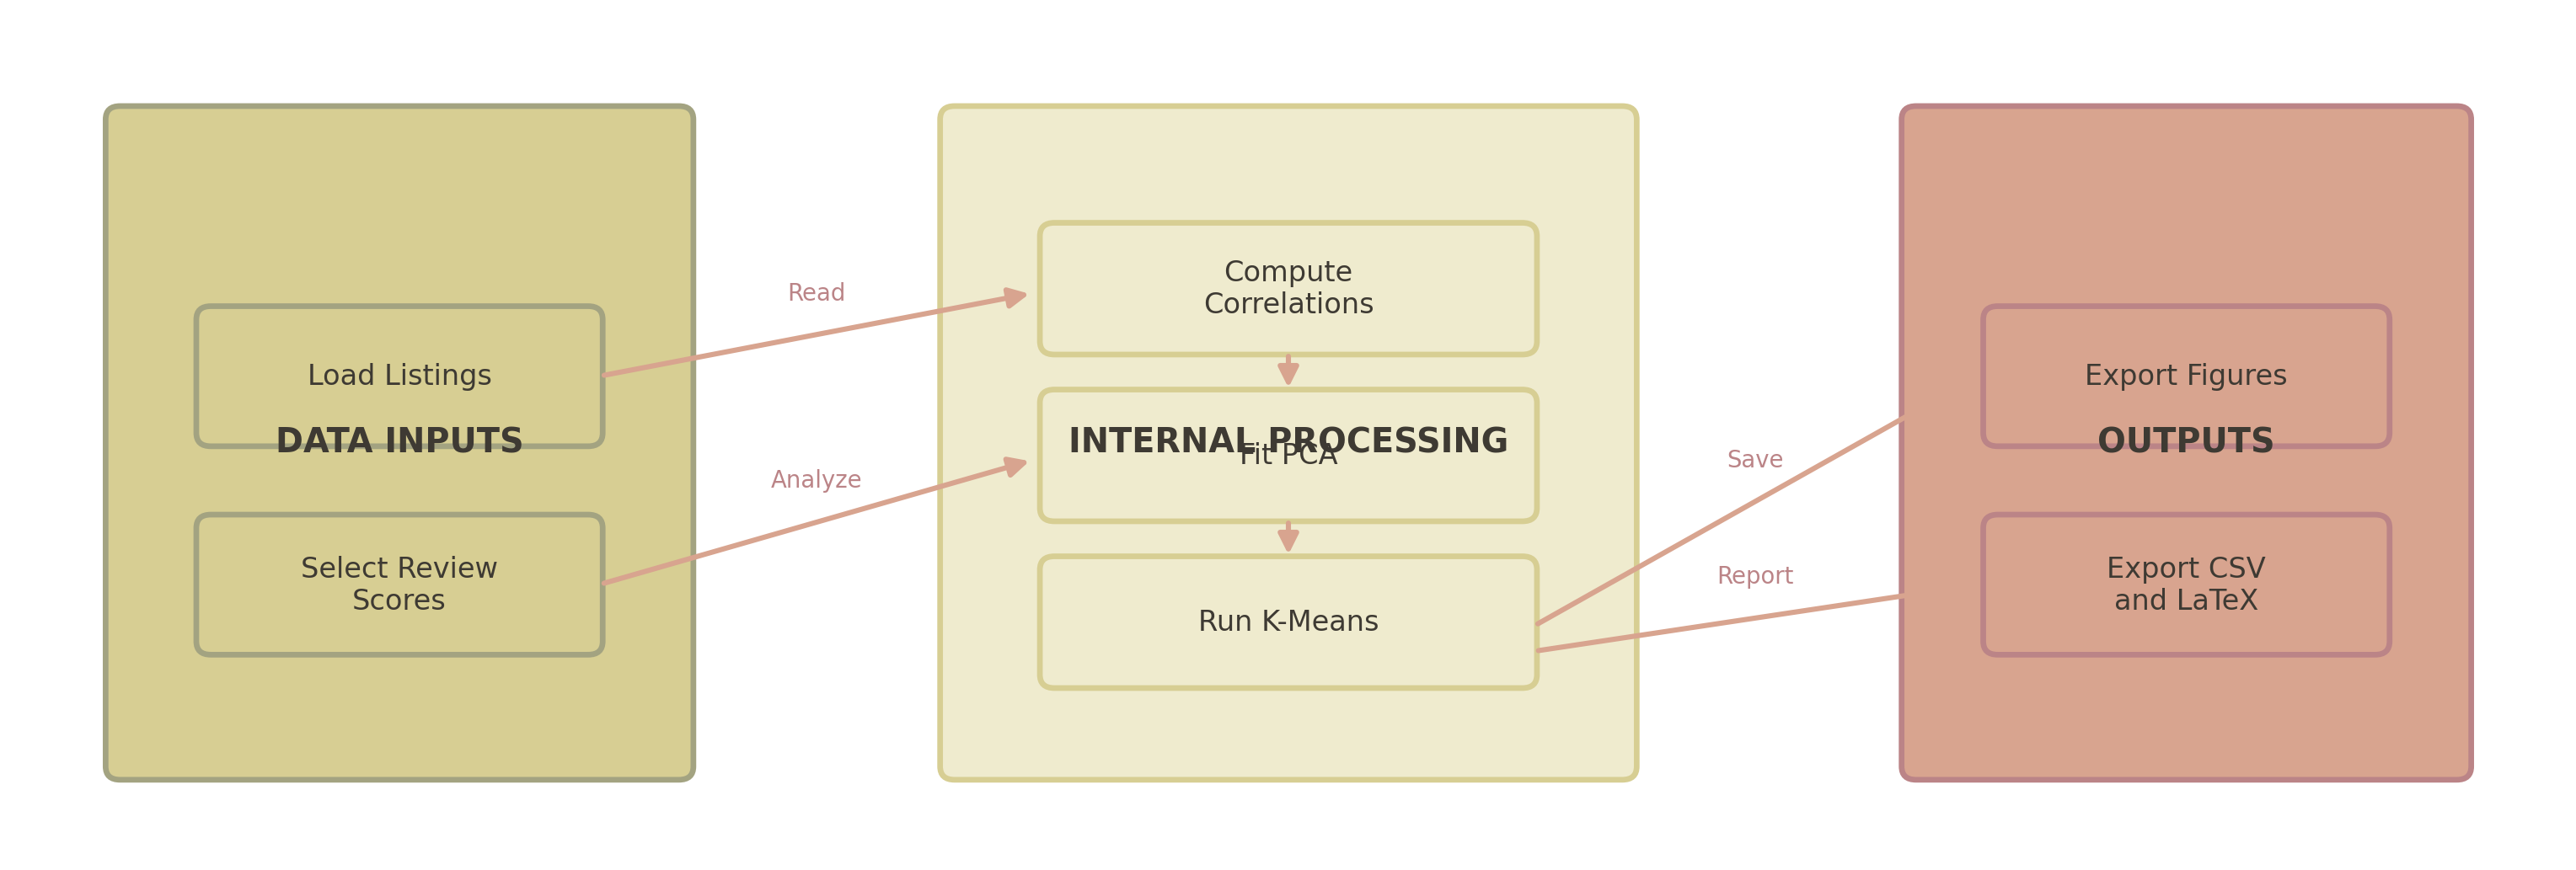
\includegraphics[width=0.98\textwidth]{p16_review_scores_correlation_pca_kmeans_mermaid.png}
    \caption{{\arabicfont\RL{مخطط سير العمل التحليلي المستخدم في هذا الدفتر.}}}
    \label{fig:p16-workflow}
\end{figure}

\section*{{\arabicfont\RL{مصفوفة الارتباط}}}
تُظهر النتائج أن جميع متغيرات التقييم ترتبط ببعضها ارتباطاً موجباً، ما يشير إلى وجود نواة تقييمية مشتركة عبر مختلف أبعاد الخبرة السكنية. وتبرز أقوى العلاقات بين الدرجة العامة والدقة \((r=0.810)\)، وبين الدرجة العامة والقيمة مقابل السعر \((r=0.810)\)، ثم بين الدقة والقيمة مقابل السعر \((r=0.771)\). وهذا يعني أن تقييم المضيف أو المسكن على أنه دقيق أو جيد القيمة يرتبط بقوة بالحكم الإجمالي المرتفع.

في المقابل، يظهر متغير الموقع بوصفه البعد الأقل اندماجاً مع بقية المتغيرات؛ إذ تتراوح ارتباطاته مع المتغيرات الأخرى بين \(0.420\) و\(0.508\). وتشير هذه النتيجة إلى أن تقييم الموقع لا يتحرك تماماً بالمنطق نفسه الذي يحكم بقية أبعاد التجربة، بل يحتفظ بدرجة من الخصوصية يمكن أن تظهر بوضوح أكبر في التحليل العاملي.

\begin{table}[H]
\centering
\caption{{\arabicfont\RL{مصفوفة الارتباط بين متغيرات درجات التقييم}}}
\label{tab:p16-correlation}
\resizebox{\textwidth}{!}{%
\begin{tabular}{lrrrrrrr}
\toprule
 & الدرجة العامة & الدقة & النظافة & تسجيل الوصول & التواصل & الموقع & القيمة \\
\midrule
الدرجة العامة   & 1.000 & 0.810 & 0.734 & 0.647 & 0.721 & 0.504 & 0.810 \\
الدقة           & 0.810 & 1.000 & 0.677 & 0.631 & 0.694 & 0.499 & 0.771 \\
النظافة         & 0.734 & 0.677 & 1.000 & 0.512 & 0.545 & 0.420 & 0.672 \\
تسجيل الوصول    & 0.647 & 0.631 & 0.512 & 1.000 & 0.708 & 0.447 & 0.600 \\
التواصل         & 0.721 & 0.694 & 0.545 & 0.708 & 1.000 & 0.461 & 0.669 \\
الموقع          & 0.504 & 0.499 & 0.420 & 0.447 & 0.461 & 1.000 & 0.508 \\
القيمة          & 0.810 & 0.771 & 0.672 & 0.600 & 0.669 & 0.508 & 1.000 \\
\bottomrule
\end{tabular}%
}
\end{table}

\begin{figure}[H]
    \centering
    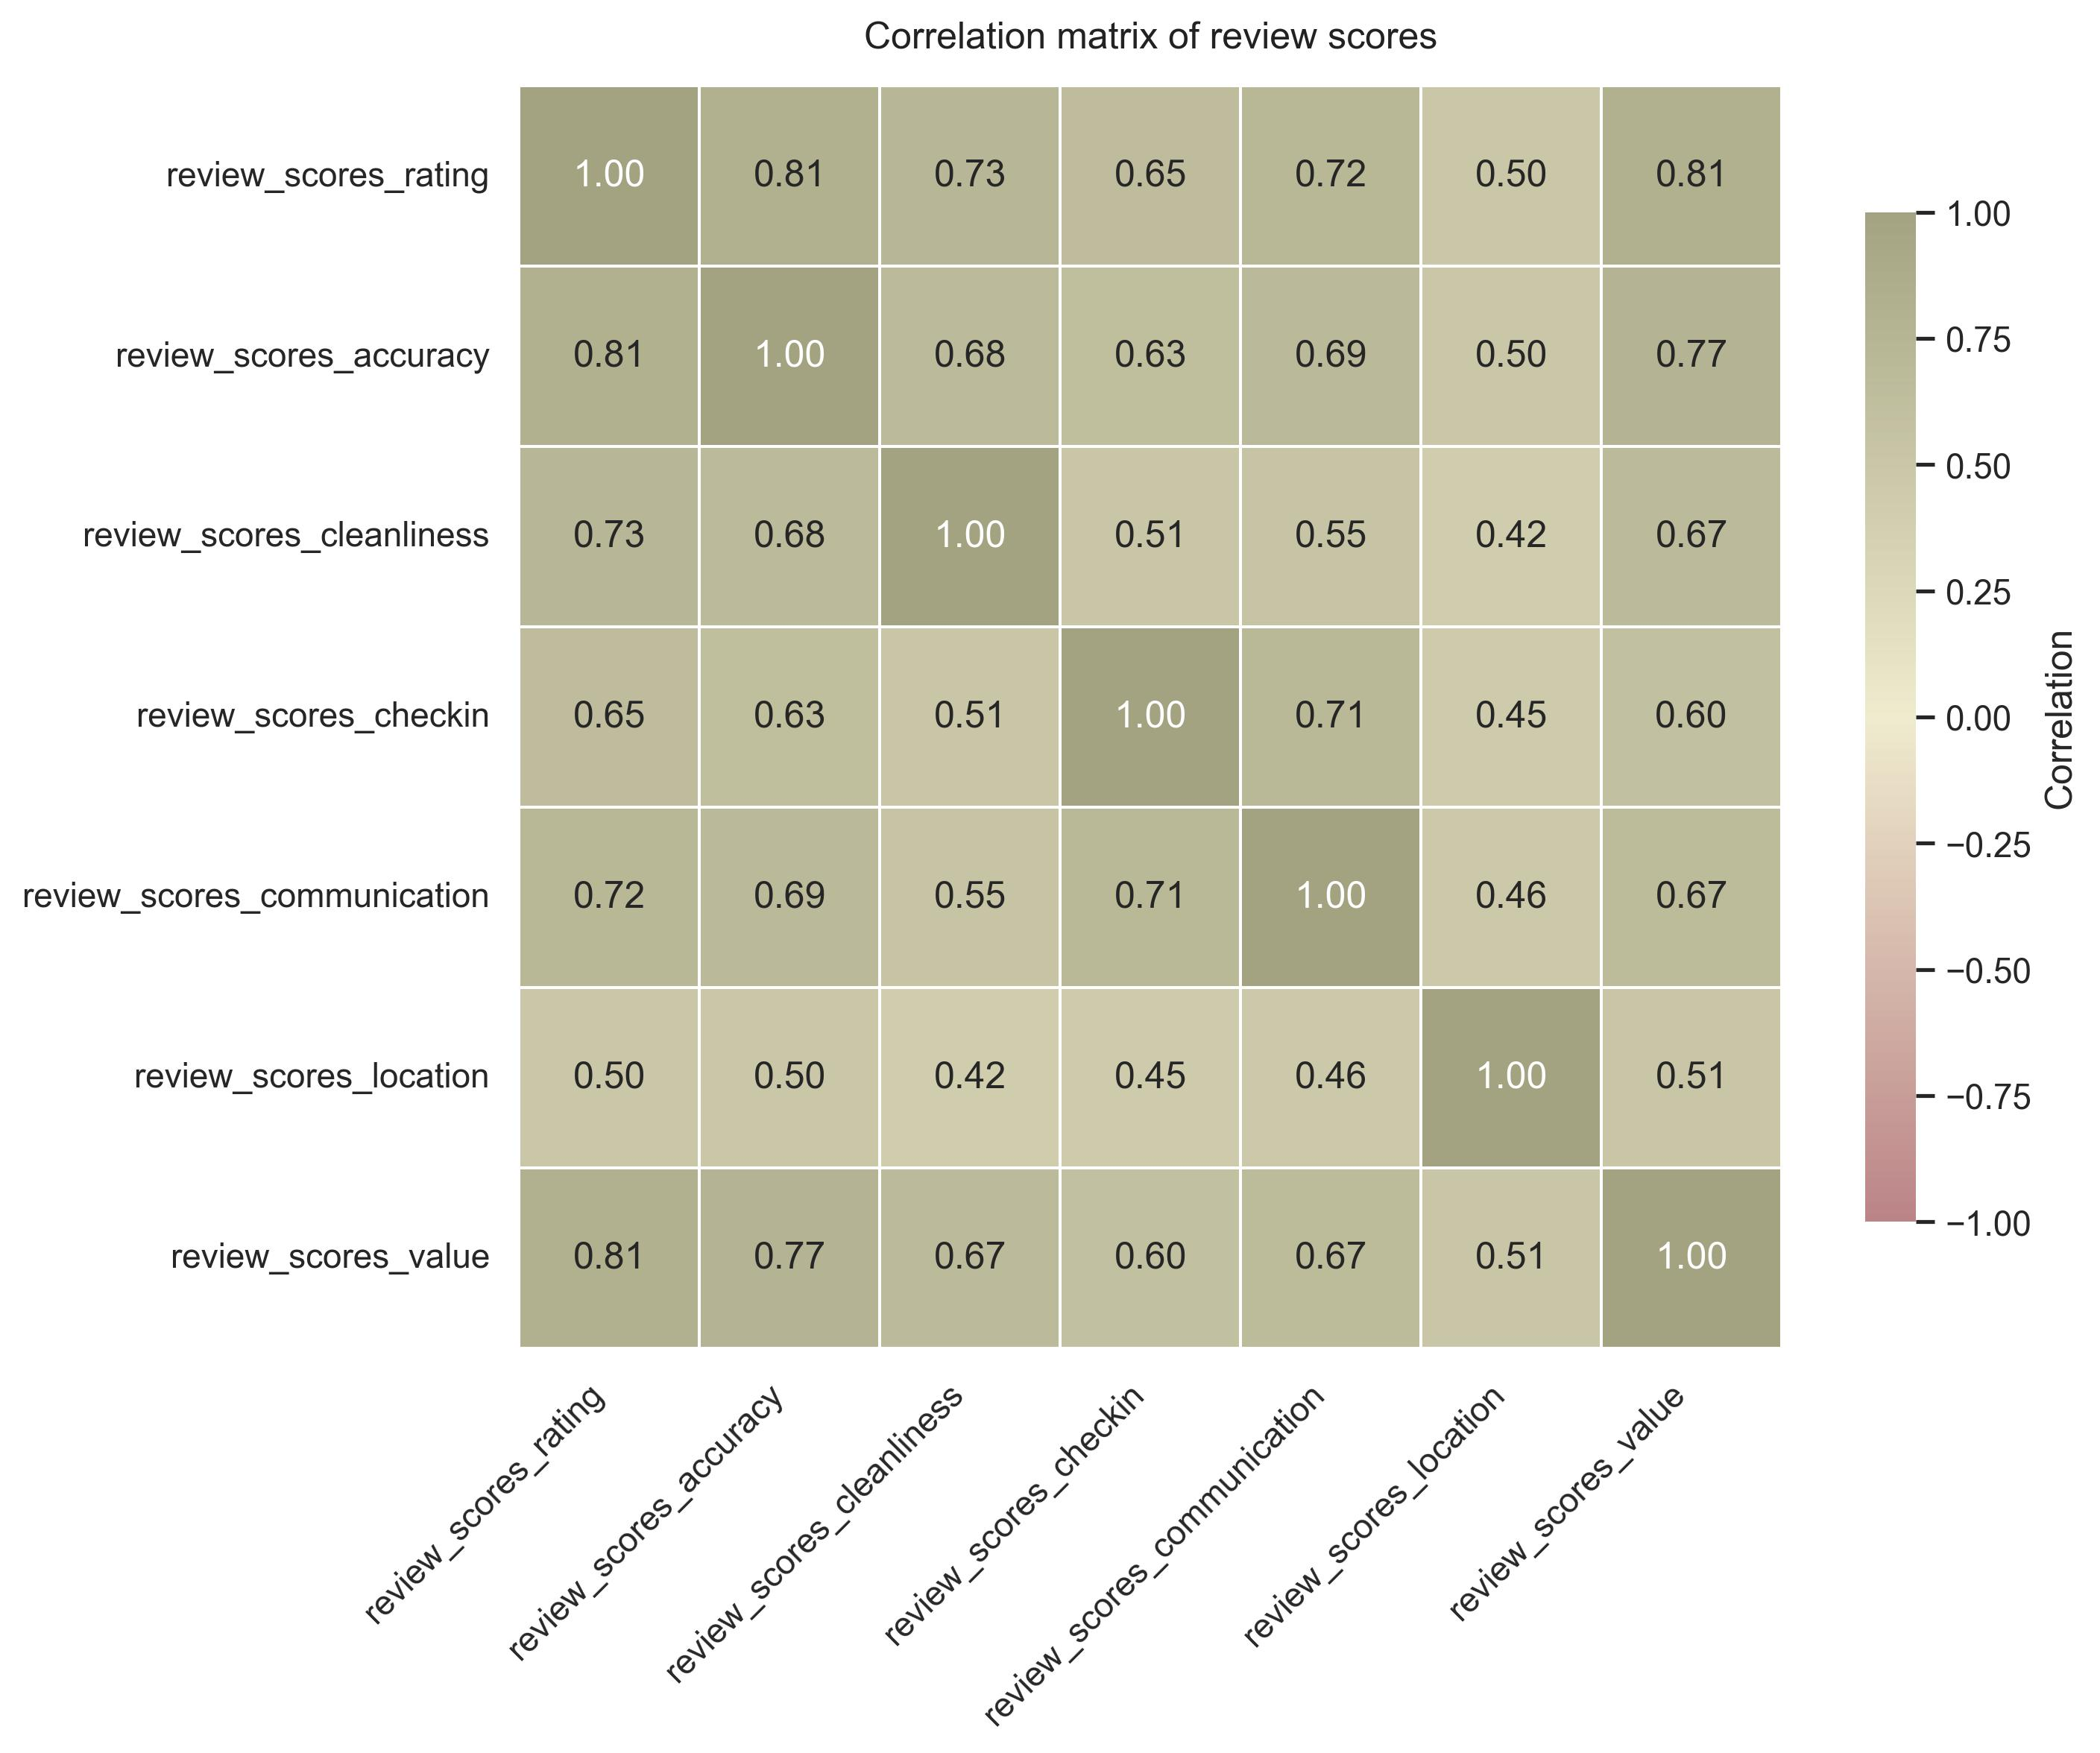
\includegraphics[width=0.92\textwidth]{p16_review_scores_corrplot.jpeg}
    \caption{{\arabicfont\RL{خريطة حرارية لمصفوفة الارتباط بين درجات التقييم.}}}
    \label{fig:p16-corrplot}
\end{figure}

\section*{{\arabicfont\RL{تحليل المكونات الرئيسية}}}
أُجري تحليل \LR{PCA} بعد توحيد متغيرات التقييم، وأظهرت نتائجه أن المكون الأول \LR{PC1} يفسر \textbf{68.16\%} من التباين الكلي، بينما ترفع إضافة المكون الثاني \LR{PC2} النسبة التراكمية إلى \textbf{77.40\%}. هذه النتيجة تعني أن الجزء الأكبر من المعلومات يمكن تلخيصه في محور أول واحد يلتقط مستوى الجودة التقييمية العامة عبر مختلف الأبعاد.

أما المكون الثاني فيفسر \textbf{9.25\%} إضافية من التباين، وهو أقل قوة بكثير من المكون الأول، لكنه مفيد تفسيرياً لأنّه يعزل بعد الموقع عن بقية المتغيرات. وهذا يفيد بأن هناك بعداً ثانوياً مستقلاً نسبياً: فقد تحصل بعض الإعلانات على تقييمات متقاربة في الجودة العامة، مع بقاء تقييم الموقع عنصراً مميزاً جزئياً داخل هذا التشابه العام.

\begin{table}[H]
\centering
\caption{{\arabicfont\RL{نسب التباين المفسَّر حسب المكونات الرئيسية}}}
\label{tab:p16-pca-variance}
\begin{tabular}{lrr}
\toprule
المكون & نسبة التباين المفسَّر & التباين التراكمي \\
\midrule
\LR{PC1} & 0.6816 & 0.6816 \\
\LR{PC2} & 0.0925 & 0.7740 \\
\LR{PC3} & 0.0823 & 0.8564 \\
\LR{PC4} & 0.0491 & 0.9055 \\
\LR{PC5} & 0.0385 & 0.9440 \\
\LR{PC6} & 0.0323 & 0.9763 \\
\LR{PC7} & 0.0237 & 1.0000 \\
\bottomrule
\end{tabular}
\end{table}

\begin{table}[H]
\centering
\caption{{\arabicfont\RL{إسهامات المتغيرات على أول مكونين رئيسيين}}}
\label{tab:p16-pca-loadings}
\begin{tabular}{lrr}
\toprule
المتغير & \LR{PC1} & \LR{PC2} \\
\midrule
الدرجة العامة   & 0.916 & -0.131 \\
الدقة           & 0.890 & -0.102 \\
النظافة         & 0.795 & -0.212 \\
تسجيل الوصول    & 0.787 &  0.005 \\
التواصل         & 0.836 & -0.044 \\
الموقع          & 0.643 &  0.752 \\
القيمة          & 0.881 & -0.081 \\
\bottomrule
\end{tabular}
\end{table}

تؤكد معاملات الإسهام أن المكون الأول يمثل بوضوح محوراً عاماً للرضا، لأن جميع المتغيرات تقريباً تحمل عليه بقيم موجبة ومرتفعة. أما المكون الثاني فتقوده قيمة الموقع \((0.752)\) بوضوح أكبر من بقية المتغيرات، وهو ما ينسجم مع ما ظهر سابقاً في مصفوفة الارتباط: الموقع مهم، لكنه ليس مندمجاً تماماً في المنظومة نفسها التي تنتظم حولها بقية درجات التقييم.

\begin{figure}[H]
    \centering
    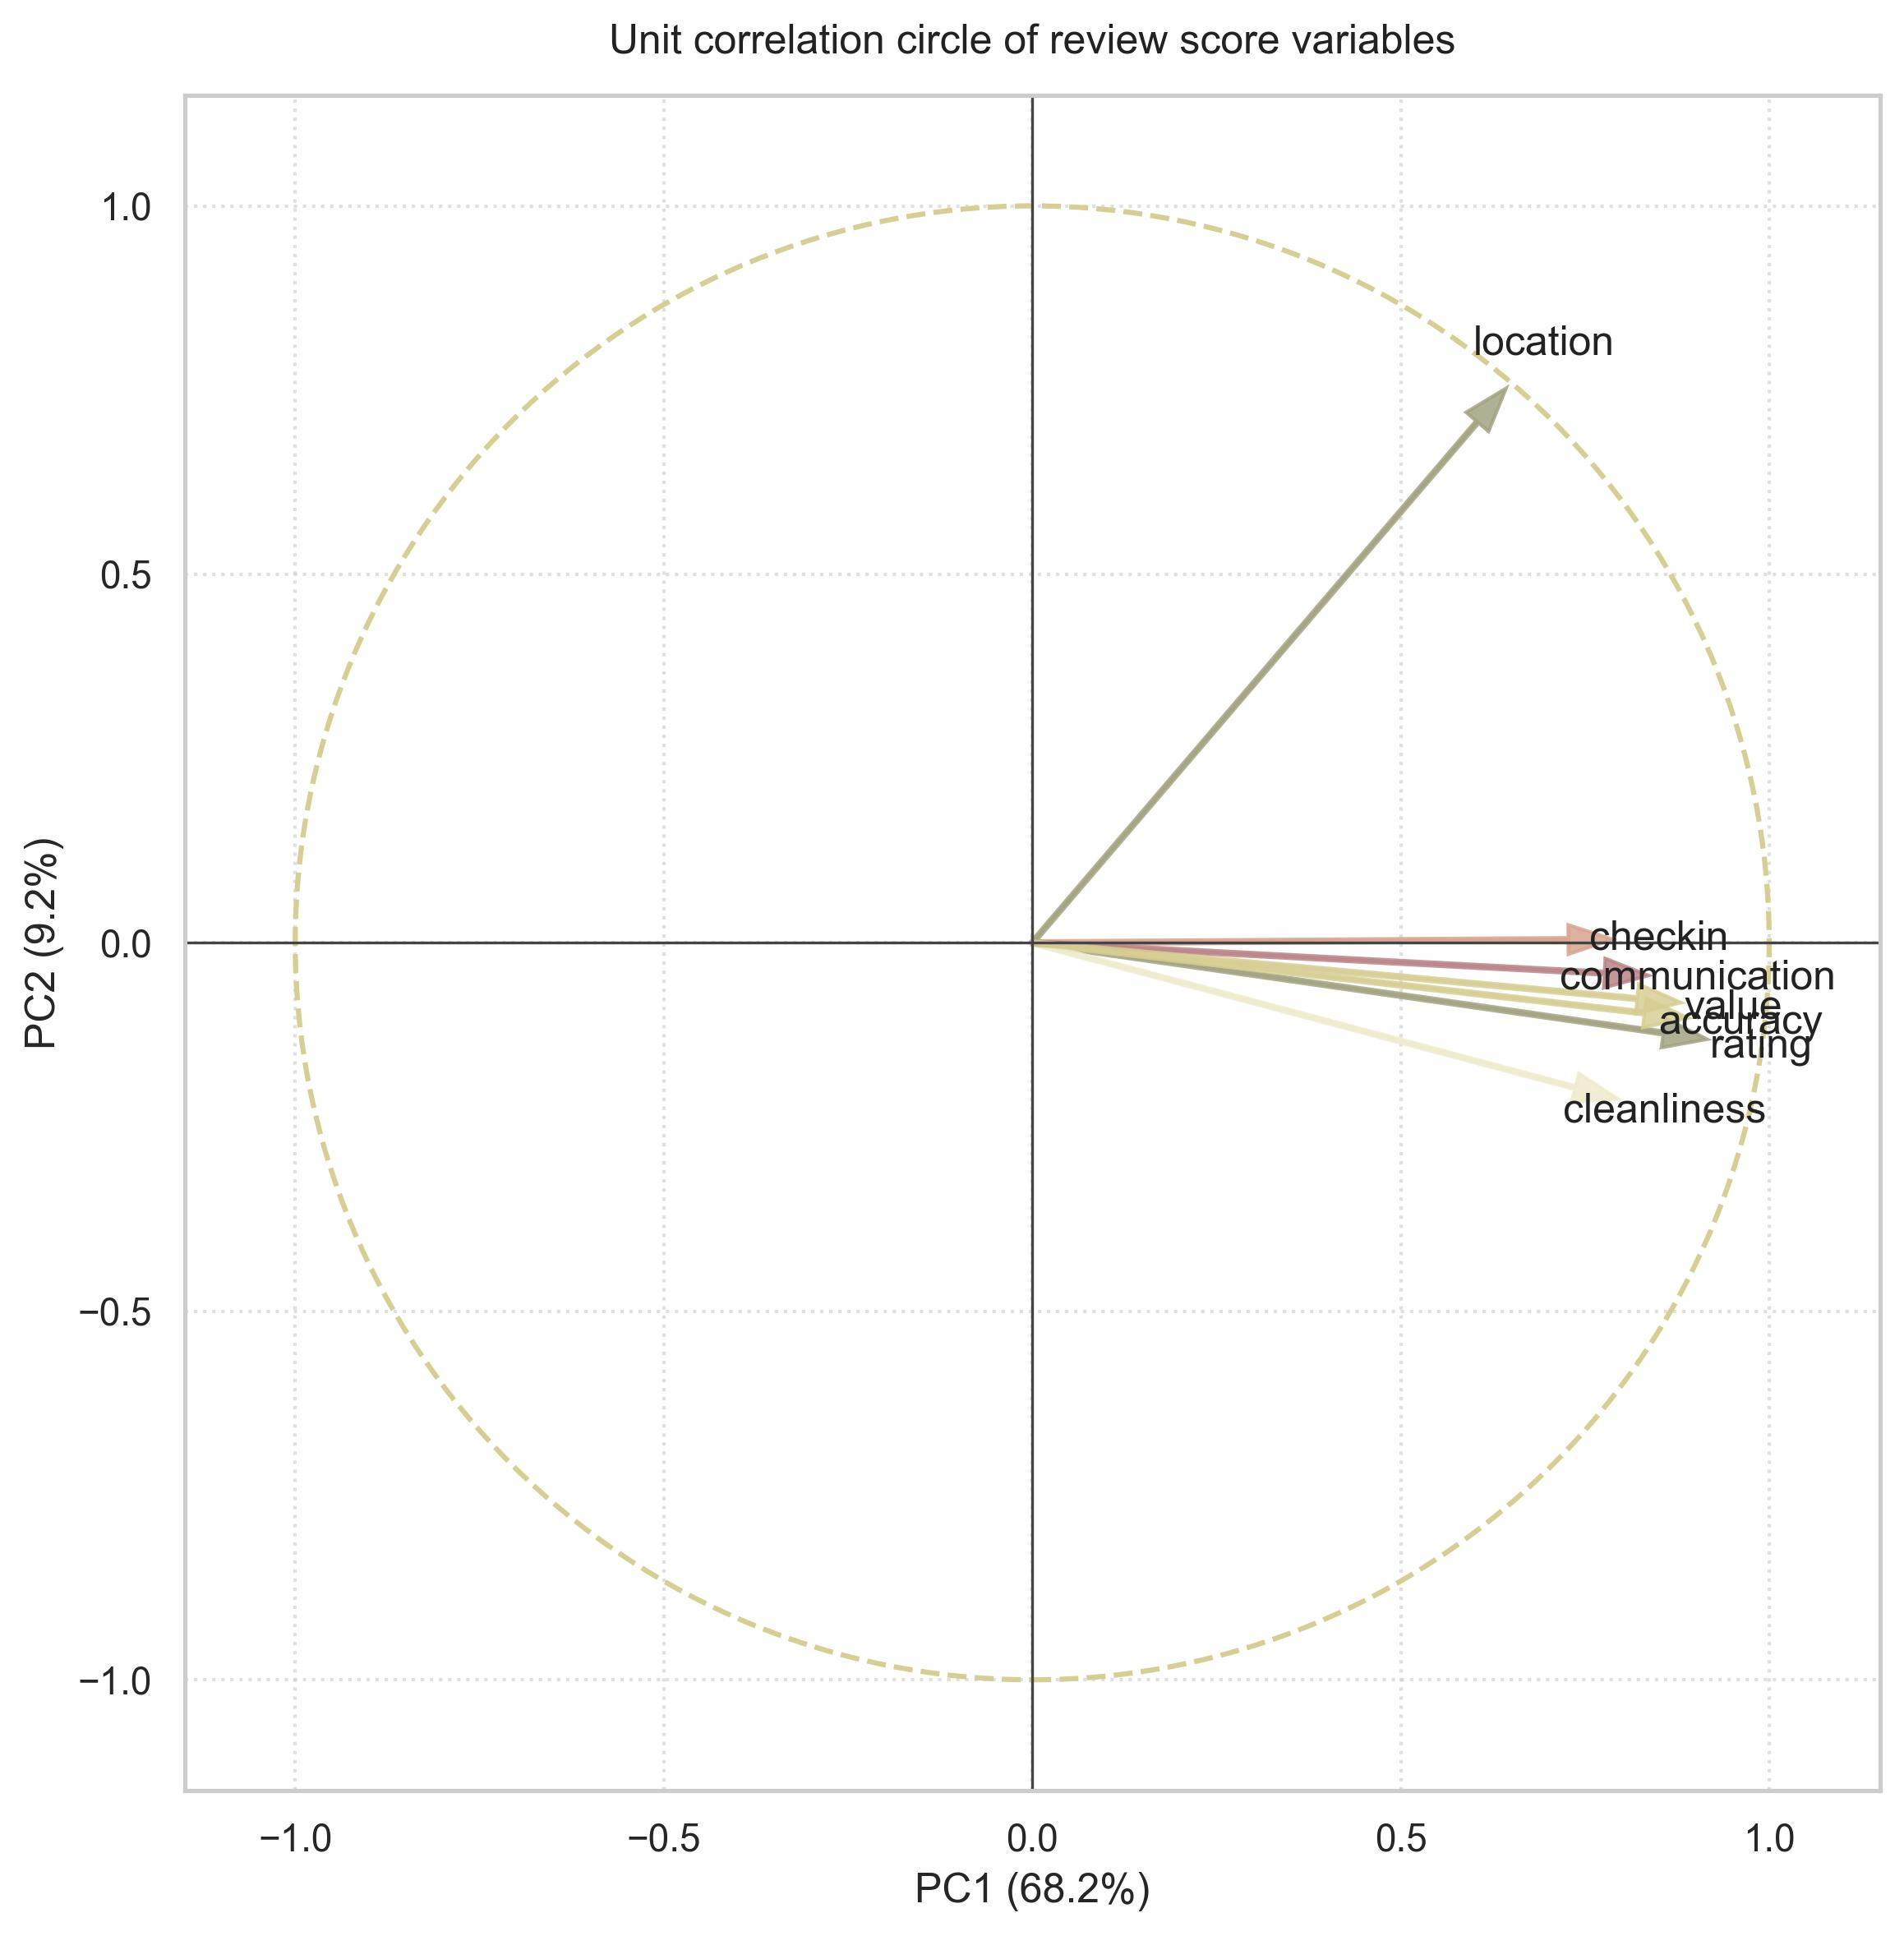
\includegraphics[width=0.82\textwidth]{p16_review_scores_pca_circle.jpeg}
    \caption{{\arabicfont\RL{الدائرة الارتباطية للمتغيرات على أول مكونين رئيسيين.}}}
    \label{fig:p16-pca-circle}
\end{figure}

\section*{{\arabicfont\RL{التجميع بطريقة \LR{K-means}}}}
طُبِّقت طريقة \LR{K-means} على الإحداثيات العاملية، وأظهرت المقارنة بين الحلول المرشحة أن أفضل تقسيم يتحقق عند \textbf{\LR{k=2}}. وتشير الجداول إلى أن هذا الحل يفصل بين كتلة كبرى جداً من الإعلانات وكتلة أصغر بكثير، بدل إنتاج تقسيمات متعددة متوازنة الحجم. ومن الناحية الجوهرية، لا يكشف هذا التقسيم عن أنماط نوعية متباينة جداً، بل عن تدرج أساسي بين إعلانات ذات مستوى تقييمي عام مرتفع نسبياً وأخرى أدنى من ذلك بوضوح.

تتكون المجموعة الأولى من \textbf{60{,}789} إعلاناً، أي نحو \textbf{95.17\%} من العينة، بينما تضم المجموعة الثانية \textbf{3{,}082} إعلاناً فقط، أي \textbf{4.83\%}. كما أن تموضع مركز المجموعة الثانية عند قيمة سالبة قوية على \LR{PC1} \((-6.9455)\) يدل على أن هذا الجزء الصغير من الإعلانات يتميز قبل كل شيء بانخفاض عام في درجات التقييم، أكثر مما يتميز ببنية داخلية مختلفة على الأبعاد الثانوية.

\begin{table}[H]
\centering
\caption{{\arabicfont\RL{درجات السيليويت للحلول المرشحة في \LR{K-means}}}}
\label{tab:p16-silhouette}
\begin{tabular}{rr}
\toprule
\LR{k} & درجة السيليويت \\
\midrule
2 & 0.7498 \\
3 & 0.5460 \\
4 & 0.4605 \\
5 & 0.4033 \\
6 & 0.4163 \\
\bottomrule
\end{tabular}
\end{table}

\begin{table}[H]
\centering
\caption{{\arabicfont\RL{أحجام المجموعات في الحل المختار عند \LR{k=2}}}}
\label{tab:p16-cluster-sizes}
\begin{tabular}{lrr}
\toprule
المجموعة & عدد الإعلانات & نسبة العينة \\
\midrule
0 & 60{,}789 & 95.17\% \\
1 & 3{,}082 & 4.83\% \\
\bottomrule
\end{tabular}
\end{table}

\begin{table}[H]
\centering
\caption{{\arabicfont\RL{مراكز المجموعات في الفضاء العاملي}}}
\label{tab:p16-centroids}
\begin{tabular}{lrrr}
\toprule
المجموعة & \LR{PC1} & \LR{PC2} & \LR{PC3} \\
\midrule
0 & 0.3532 & -0.0109 & 0.0064 \\
1 & -6.9455 & 0.2138 & -0.1252 \\
\bottomrule
\end{tabular}
\end{table}

\begin{figure}[H]
    \centering
    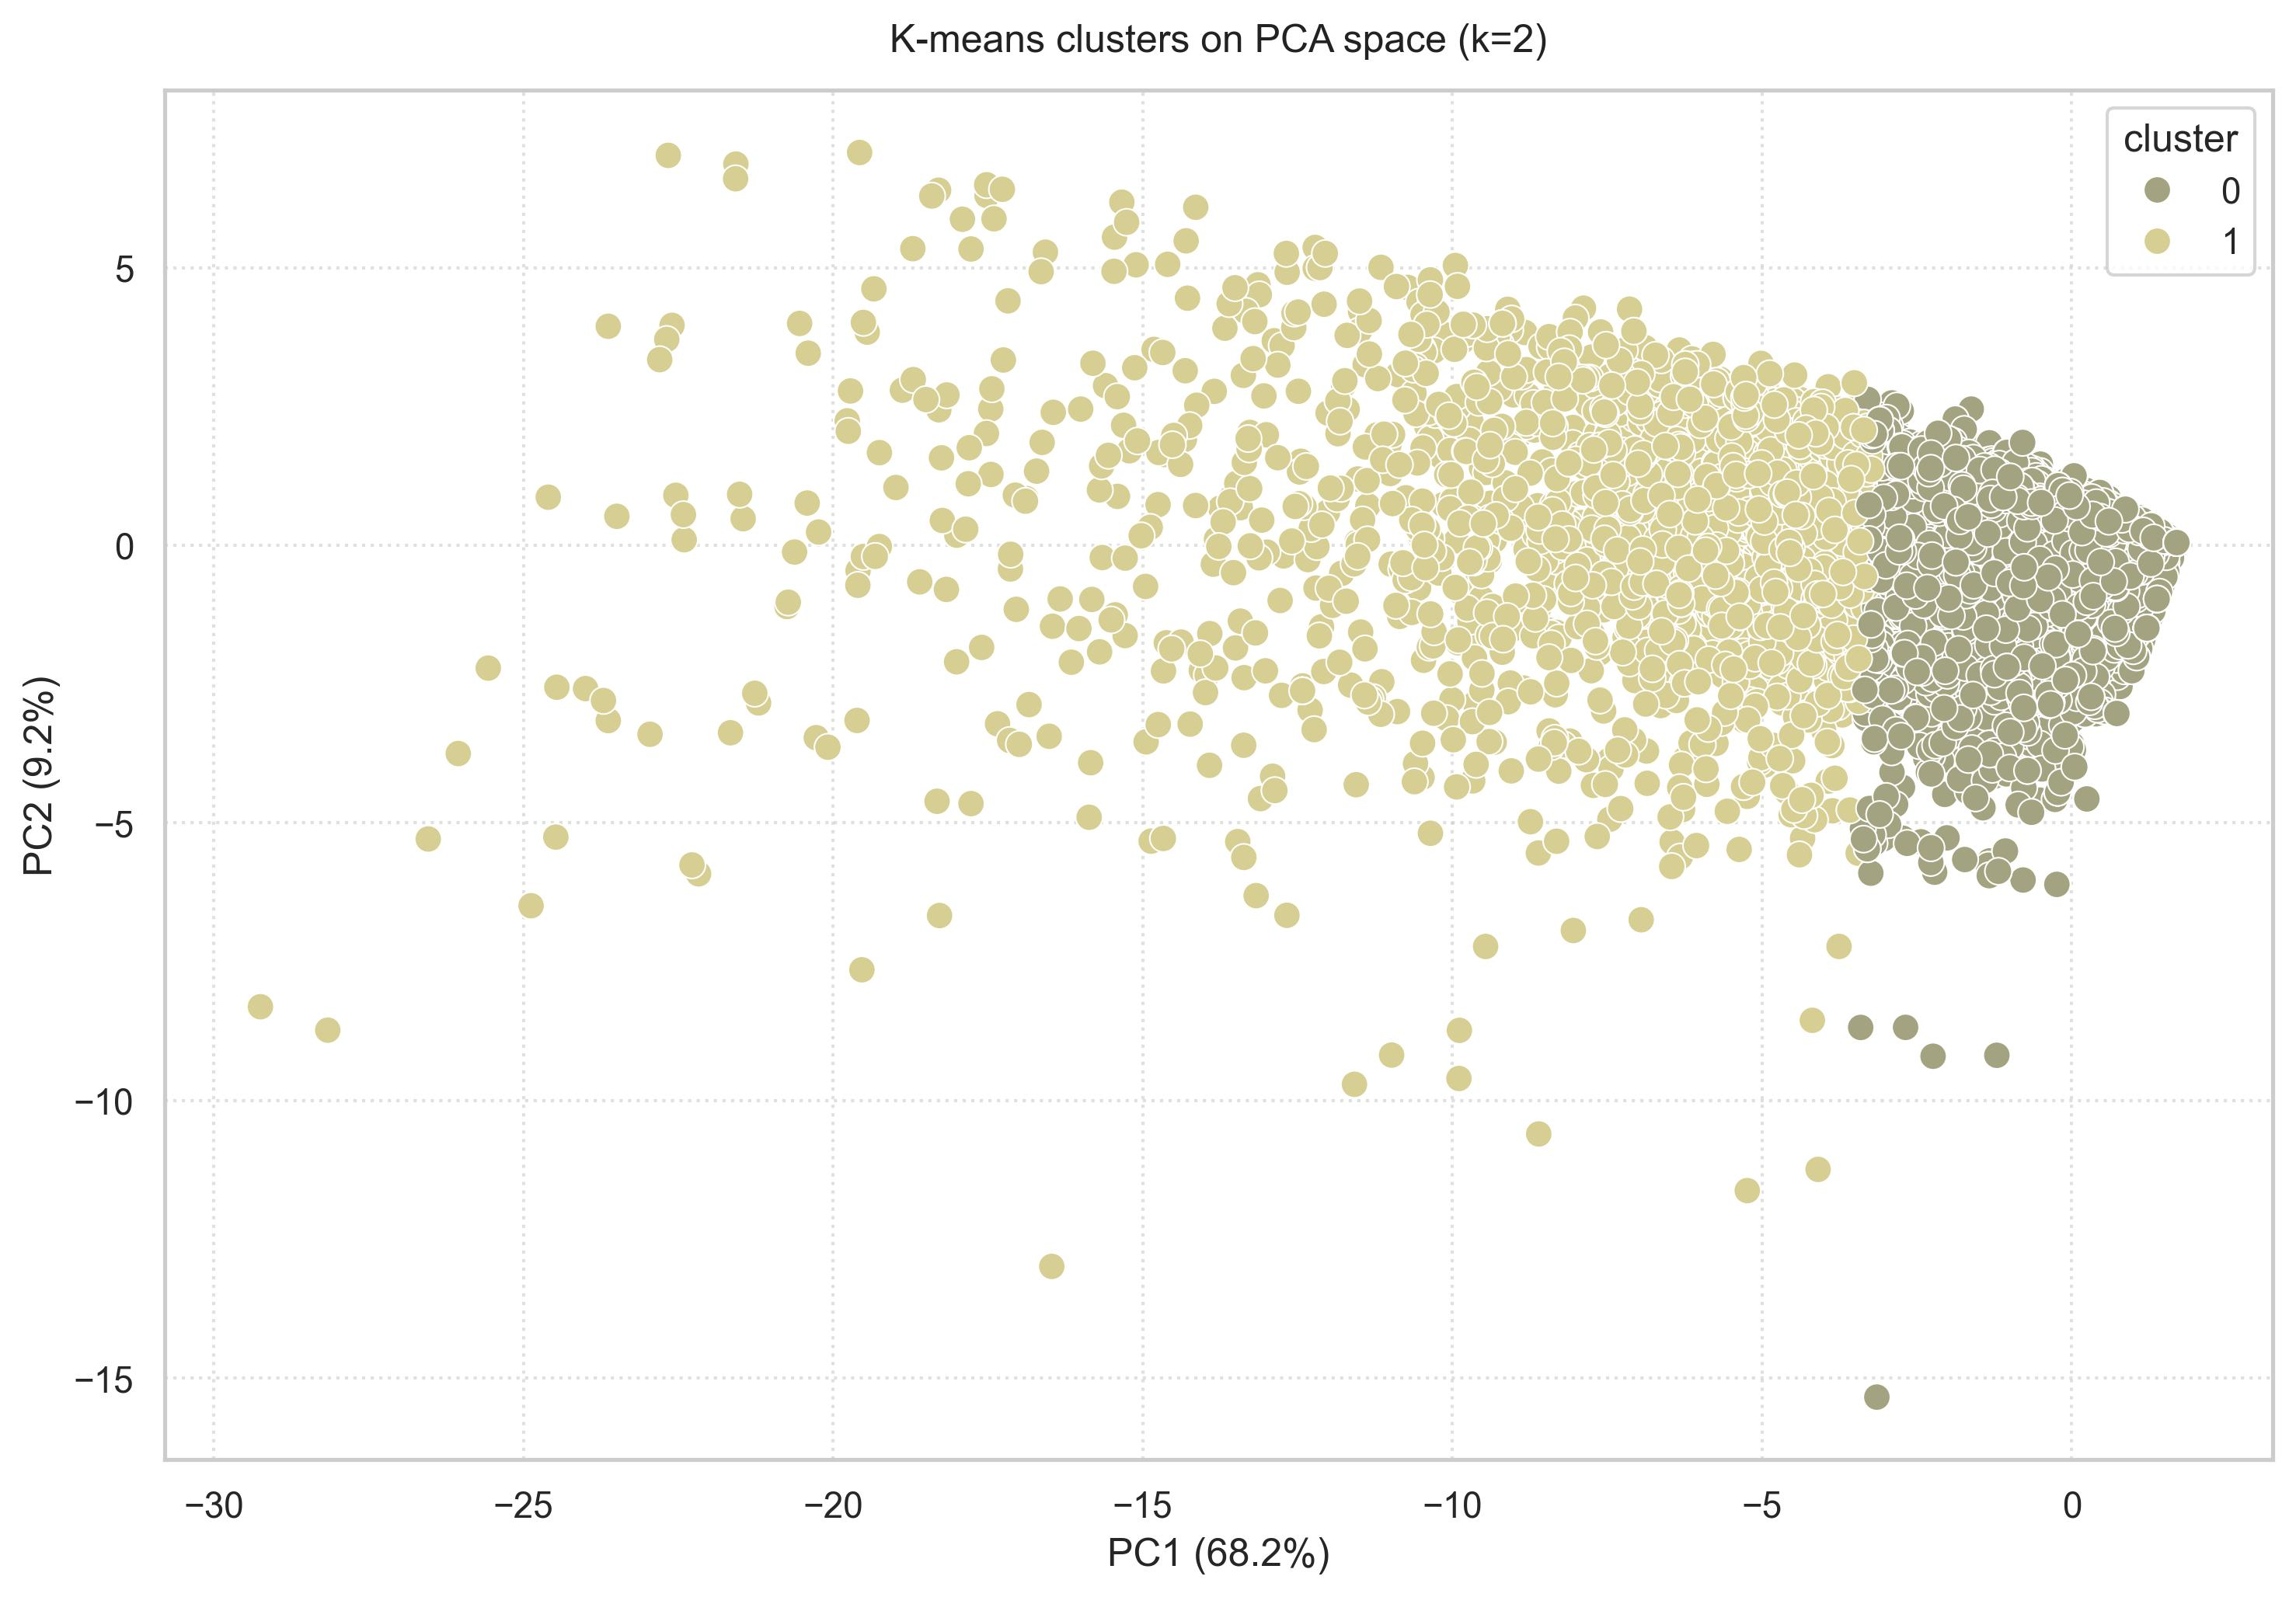
\includegraphics[width=0.95\textwidth]{p16_review_scores_kmeans_clusters.jpeg}
    \caption{{\arabicfont\RL{تمثيل المجموعات في المستوى المحدد بالمكونين الأول والثاني.}}}
    \label{fig:p16-kmeans}
\end{figure}

\section*{{\arabicfont\RL{خلاصة تفسيرية}}}
تُظهر النتائج أن نظام درجات التقييم في هذه البيانات شديد الاتساق الداخلي، وأن أغلب أبعاده تتحرك معاً ضمن محور عام واحد للرضا. ويعني ذلك أن الانتقال من تقييمات منخفضة إلى تقييمات مرتفعة لا يحدث عادةً في بعد منفرد فقط، بل ينعكس غالباً على الدقة والنظافة والتواصل والقيمة في الوقت نفسه.

في المقابل، يبقى الموقع بعداً أقل اندماجاً من غيره، وهو ما يمنحه وزناً تفسيرياً خاصاً في المكون الثاني. أما التحليل التجميعي فيبين أن الانقسام الأوضح تجريبياً ليس بين أنماط متعددة معقدة، بل بين أغلبية واسعة من الإعلانات ذات تقييمات جيدة نسبياً وأقلية صغيرة تبدو أقل جودة على المحور التقييمي العام. وبناءً على ذلك، يمكن قراءة هذه البنية على أنها هيمنة لبعد جودة شامل، مع احتفاظ الموقع بهامش من الاستقلال النسبي.

\section*{{\arabicfont\RL{ملحق: الحصيلة الكربونية للتشغيل}}}
يعرض هذا الملحق البصمة الكربونية المسجلة فعلياً أثناء تنفيذ الدفتر. وقد استُخرجت القيم من ملف التقرير الكربوني الموحد للمشروع، وبالتالي فهي لا تمثل تقديراً نظرياً بل أثراً حسابياً محفوظاً في ملفات الخرج.

\begin{table}[H]
\centering
\caption{{\arabicfont\RL{الحصيلة الكربونية المسجلة لتنفيذ الدفتر}}}
\label{tab:p16-carbon}
\begin{tabular}{p{0.28\textwidth}p{0.58\textwidth}}
\toprule
المؤشر & القيمة \\
\midrule
اسم الدفتر المنفذ & \LR{p16\_review\_scores\_correlation\_pca\_kmeans.ipynb} \\
عدد الملاحظات المعالجة & 63{,}871 \\
تاريخ التنفيذ & 2026-04-17 19:56:50 \\
زمن التنفيذ & 364.81 ثانية \\
إجمالي الاستهلاك الكهربائي & 0.035468 \LR{kWh} \\
إجمالي الانبعاثات & 1.78 غرام \LR{eCO\textsubscript{2}} \\
\bottomrule
\end{tabular}
\end{table}

وتشير هذه القيم إلى أن التحليل، رغم معالجته لعينة كبيرة نسبياً، ظل محدود الكلفة الطاقية والانبعاثية. وهذا ينسجم مع طبيعة المعالجة الإحصائية المعتمدة هنا، والتي تعتمد أساساً على مصفوفات رقمية ورسوم وصفية دون الحاجة إلى تدريب نموذج ثقيل أو إلى استدعاءات خارجية مكثفة.

\end{RTL}

\end{document}
